\chapter{Technical Implementation}
\label{chap:technical-implementation}


This section details the technical execution of the system, covering data management, AI model integration, backend architecture, and deployment strategies.

% --------------------------------------------
\section{Data Collection and Management}

\subsection{Data Sources}

The system integrates data from six primary sources to provide comprehensive urban mobility services:

\begin{table}[H]
    \centering
    \renewcommand{\arraystretch}{1.3}
    \begin{tabularx}{\textwidth}{|p{3.5cm}|p{2.5cm}|X|}
        \hline
        \textbf{Source} & \textbf{Type} & \textbf{Data Collected} \\
        \hline
        \href{https://giaothong.hochiminhcity.gov.vn}{HCMC Traffic Portal} & Live API & Real-time camera images from 702 traffic cameras across the city \\
        \hline
        TomTom API & Commercial API & Geocoding services, turn-by-turn routing, and location search \\
        \hline
        \href{https://busmap.vn}{HCMC Bus Map} & Enterprise Data & Official bus routes, stop locations \\
        \hline
        Groq API & LLM Service & Natural language processing for trip planning queries \\
        \hline
        Custom Dataset & Manual Curation & Curated database of restaurants, hotels, and landmarks \\
        \hline
    \end{tabularx}
    \caption{Data Sources and Their Contributions}
    \label{tab:data-sources}
\end{table}

\subsection{Database Architecture}

The system employs a hybrid database strategy, using MySQL for user-related data requiring ACID compliance and SQLite for high-volume detection results requiring fast writes.

\paragraph{MySQL Database: User Management}

The MySQL database manages all user-related data with the following tables:

\begin{itemize}[noitemsep]
    \item \textbf{users}: Stores user credentials including username, hashed password (bcrypt), email, and OAuth provider information. Supports multiple authentication methods (local, Google, GitHub).
    
    \item \textbf{saved\_locations}: User's bookmarked places with name, coordinates, address, and creation timestamp.
    
    \item \textbf{route\_history}: Records of previously calculated routes including origin, destination, route type (car/bus), distance, duration, and polyline geometry.
    
    \item \textbf{trip\_history}: AI-generated trip itineraries with full JSON data, creation date, and associated images.
    
    \item \textbf{sos\_reports}: Emergency reports containing location, description, category (accident, breakdown, hazard), images, reporter ID, and status (active/resolved/hidden).
    
    \item \textbf{sos\_comments}: Community comments on SOS reports with spam detection flags.
    
    \item \textbf{sos\_user\_blocks}: Spam prevention table tracking blocked users and block expiration.
\end{itemize}

\paragraph{SQLite Database: Detection Results}

The SQLite database (\texttt{detections.db}) stores vehicle detection results optimized for time-series queries:

\begin{itemize}[noitemsep]
    \item \textbf{Table}: \texttt{detections} --- stores detection results per camera image
    \item \textbf{Fields}: image\_path (unique), camera\_id, camera\_name, timestamp, vehicle counts by type (car, motorcycle, bus, truck), total count, processing time, optimization method used
    \item \textbf{Indexes}: Compound index on (camera\_id, timestamp) for efficient time-range queries; separate indexes on camera\_id and timestamp for flexibility
    \item \textbf{Rationale}: SQLite chosen over MySQL for detection data due to simpler deployment, faster bulk inserts during batch processing, and self-contained file-based storage
\end{itemize}

\paragraph{JSON Data Files}

Several datasets are stored as JSON files for fast loading and easy updates:

\begin{itemize}[noitemsep]
    \item \textbf{camera\_locations.json}: Camera network metadata (702 cameras) with ID, name, coordinates, and display name. Updated when new cameras are added to the traffic portal.
    
    \item \textbf{combined\_locations.json}: Places database ($\sim$700 locations) organized by category (restaurants, hotels, landmarks) with name, coordinates, normalized name for fuzzy matching, and local image path.
    
    \item \textbf{segment\_thresholds.json}: Pre-computed percentile thresholds (P50, P80) for each road segment based on historical vehicle counts, used for congestion classification.
    
    \item \textbf{segment\_geometries.geojson}: Road segment geometries in GeoJSON format for map visualization and camera-to-segment mapping.
\end{itemize}

\paragraph{CSV Data Files (Bus Network)}

Bus network data is stored in CSV format for compatibility with pandas:

\begin{itemize}[noitemsep]
    \item \textbf{stops.csv}: 4,343 bus stops with stopId, stopName, latitude, longitude
    \item \textbf{routes.csv}: 127 bus routes with routeId, busNumber, fare, headway (minutes between buses)
    \item \textbf{trips.csv}: 5,184 trip segments linking routes to stops with sequence order and distance to next stop
\end{itemize}

\subsection{Caching Strategy}

To minimize startup time and repeated computation, the system implements pickle-based caching:

\begin{itemize}[noitemsep]
    \item \textbf{Bus Graph Cache}: Serialized NetworkX MultiDiGraph with 1,500 nodes and $\sim$10,000 edges. First build takes 10-30 seconds; cached load takes $<$1 second.
    
    \item \textbf{Fuzzy Match Cache}: Pre-built token index for place name matching. Eliminates 2-3 second index build time on each request.
    
    \item \textbf{Cache Invalidation}: Caches are automatically rebuilt when source data files are modified (detected via file modification timestamps).
\end{itemize}

% --------------------------------------------
\section{AI Model Integration}

\subsection{YOLOv11 Vehicle Detection}

The vehicle detection pipeline uses YOLOv11 Large model pretrained on COCO dataset:

\paragraph{Model Configuration}
\begin{itemize}[noitemsep]
    \item \textbf{Input}: 960×540 pixel traffic camera images
    \item \textbf{Target Classes}: car (class 2), motorcycle (class 3), bus (class 5), truck (class 7)
    \item \textbf{Class-Specific Thresholds}: Optimized per-class confidence thresholds to handle varying object sizes (motorcycle: 0.15, car: 0.25, truck: 0.30, bus: 0.38)
\end{itemize}

\paragraph{Image Preprocessing}
\begin{enumerate}[noitemsep]
    \item Convert to LAB color space
    \item Apply CLAHE (Contrast Limited Adaptive Histogram Equalization) on L channel with clipLimit=2.5, tileGridSize=8×8
    \item Convert back to BGR
    \item Apply mild denoising using fastNlMeansDenoisingColored
\end{enumerate}

\paragraph{Deployment Options}
\begin{itemize}[noitemsep]
    \item \textbf{Local}: Direct inference using Ultralytics library on CPU/GPU
    \item \textbf{Cloud}: Modal serverless deployment with NVIDIA T4 GPU, providing 5-10× speedup over CPU inference
\end{itemize}

\subsection{Groq LLM Integration}

The trip planning feature uses Groq's hosted LLM service:

\begin{itemize}[noitemsep]
    \item \textbf{Model}: llama-3.3-70b-versatile (70 billion parameters)
    \item \textbf{Input}: Natural language trip request with HCMC context
    \item \textbf{Output}: Structured JSON with place names, visit times, durations, and descriptions
    \item \textbf{Prompt Engineering}: System prompt includes HCMC geography context, output format requirements, and examples of valid responses
    \item \textbf{Response Time}: 1-2 seconds for typical queries
\end{itemize}

\subsection{RapidFuzz Text Matching}

Fuzzy string matching bridges LLM output to the places database:

\begin{itemize}[noitemsep]
    \item \textbf{Preprocessing}: Unicode normalization (unidecode), lowercase conversion, punctuation removal
    \item \textbf{Scoring}: Weighted combination of token\_set\_ratio (50\%), partial\_ratio (25\%), and token\_sort\_ratio (25\%)
    \item \textbf{Optimization}: Token-based inverted index for O(1) candidate retrieval instead of O(n) full scan
    \item \textbf{Threshold}: Minimum 70\% similarity score required for a valid match
    \item \textbf{Aliases}: Manual alias map for common name variations (e.g., ``Independence Palace'' → ``Dinh Độc Lập'')
\end{itemize}

% --------------------------------------------
\section{Backend Architecture}

\subsection{Flask Application Structure}

The backend is built on Flask 3.0 with the following organization:

\begin{itemize}[noitemsep]
    \item \textbf{API.py}: Main application file containing all route handlers
    \item \textbf{Authentication}: JWT-based token authentication with 24-hour expiration; OAuth 2.0 support for Google, GitHub.
    \item \textbf{CORS}: Enabled for cross-origin requests from frontend applications
    \item \textbf{Error Handling}: Consistent JSON error responses with appropriate HTTP status codes
\end{itemize}

\subsection{Core API Modules}

\paragraph{Authentication Module}
\begin{itemize}[noitemsep]
    \item User registration with bcrypt password hashing
    \item Login with JWT token generation
    \item OAuth flow handling for social login providers
    \item Token validation decorator for protected routes
\end{itemize}

\paragraph{Routing Module}
\begin{itemize}[noitemsep]
    \item TomTom API integration for car/walking routes
    \item Custom A* implementation for bus routing
    \item Route polyline decoding and map generation with Folium
    \item Distance and duration calculations
\end{itemize}

\paragraph{Detection Module}
\begin{itemize}[noitemsep]
    \item Camera image retrieval from HCMC traffic portal
    \item Local or Modal-based YOLO inference
    \item Result aggregation and database storage
    \item Segment-level vehicle count calculation
\end{itemize}

\paragraph{Congestion Module}
\begin{itemize}[noitemsep]
    \item Real-time segment aggregation from detection results
    \item Percentile-based threshold calculation
    \item GeoJSON generation with congestion colors
    \item Historical data querying for trend analysis
\end{itemize}

\paragraph{Trip Planning Module}
\begin{itemize}[noitemsep]
    \item Groq API communication with structured prompts
    \item Fuzzy matching pipeline for place resolution
    \item TomTom routing between itinerary stops
    \item Map generation with markers and route polylines
\end{itemize}

\paragraph{SOS Module}
\begin{itemize}[noitemsep]
    \item Incident report creation with image upload
    \item Geospatial querying for nearby reports
    \item Comment system with spam detection
    \item Report lifecycle management (active → resolved → hidden)
\end{itemize}

\subsection{Key API Endpoints}

\begin{table}[H]
    \centering
    \renewcommand{\arraystretch}{1.2}
    \footnotesize
    \begin{tabularx}{\textwidth}{|p{1.2cm}|p{4.5cm}|X|}
        \hline
        \textbf{Method} & \textbf{Endpoint} & \textbf{Description} \\
        \hline
        POST & /api/auth/register & Create new user account \\
        \hline
        POST & /api/auth/login & Authenticate and receive JWT \\
        \hline
        POST & /api/auth/google & Google OAuth authentication \\
        \hline
        POST & /search & Search locations within HCMC \\
        \hline
        POST & /route & Calculate car/walking route \\
        \hline
        GET & /api/bus/route & Calculate optimal bus route \\
        \hline
        POST & /api/groq & Generate AI trip itinerary \\
        \hline
        GET & /api/cameras & List all traffic cameras \\
        \hline
        POST & /api/detect/route-cameras & Run detection on route cameras \\
        \hline
        GET & /api/congestion/geojson & Get congestion map data \\
        \hline
        POST & /api/sos & Submit emergency report \\
        \hline
        GET & /api/sos/nearby & Get reports near location \\
        \hline
    \end{tabularx}
    \caption{Key API Endpoints}
    \label{tab:api-endpoints}
\end{table}

% --------------------------------------------
\section{Cloud Deployment}

\subsection{Modal Serverless GPU}

For production-grade vehicle detection, the system uses Modal for serverless GPU inference:

\begin{itemize}[noitemsep]
    \item \textbf{Platform}: Modal (modal.com) serverless compute
    \item \textbf{GPU}: NVIDIA T4 (16GB VRAM) with automatic scaling
    \item \textbf{Container}: Custom Debian-based image with Ultralytics, OpenCV, PyTorch
    \item \textbf{Model Storage}: Persistent volume for YOLO weights (avoids re-download)
    \item \textbf{Endpoint}: FastAPI-based REST endpoint for batch inference
    \item \textbf{Latency}: $\sim$100ms per image (vs $\sim$500ms on CPU)
    \item \textbf{Cost}: Pay-per-use pricing, no idle charges
\end{itemize}

\subsection{Fallback Strategy}

The system implements graceful degradation when Modal is unavailable:

\begin{enumerate}[noitemsep]
    \item Attempt Modal API call with 30-second timeout
    \item On failure, fall back to local CPU inference
    \item Log fallback event for monitoring
    \item Return results with ``optimization\_used'' field indicating method
\end{enumerate}


% --------------------------------------------

\section{Frontend}

The frontend is built as a single-page application (SPA) using React.js with Material-UI for consistent design.

\subsection{Framework and Libraries}

\begin{table}[H]
    \centering
    \renewcommand{\arraystretch}{1.3}
    \begin{tabularx}{\textwidth}{|p{3cm}|p{2.5cm}|X|}
        \hline
        \textbf{Framework} & \textbf{Version} & \textbf{Purpose} \\
        \hline
        React & 18.x & Component-based UI framework with hooks for state management \\
        \hline
        Material-UI & v4 & Pre-built UI components, theming, and responsive design \\
        \hline
        React Router & v6 & Client-side routing and navigation between pages \\
        \hline
        Goong Maps JS & Latest & Vietnam-optimized interactive map rendering \\
        \hline
        Day.js & Latest & Lightweight date/time formatting with timezone support \\
        \hline
        Axios/Fetch & - & HTTP client for API communication \\
        \hline
    \end{tabularx}
    \caption{Frontend Framework Stack}
\end{table}

\subsection{Application Screenshots}

The following screenshots demonstrate the key features of the web application:

\begin{figure}[H]
    \centering
    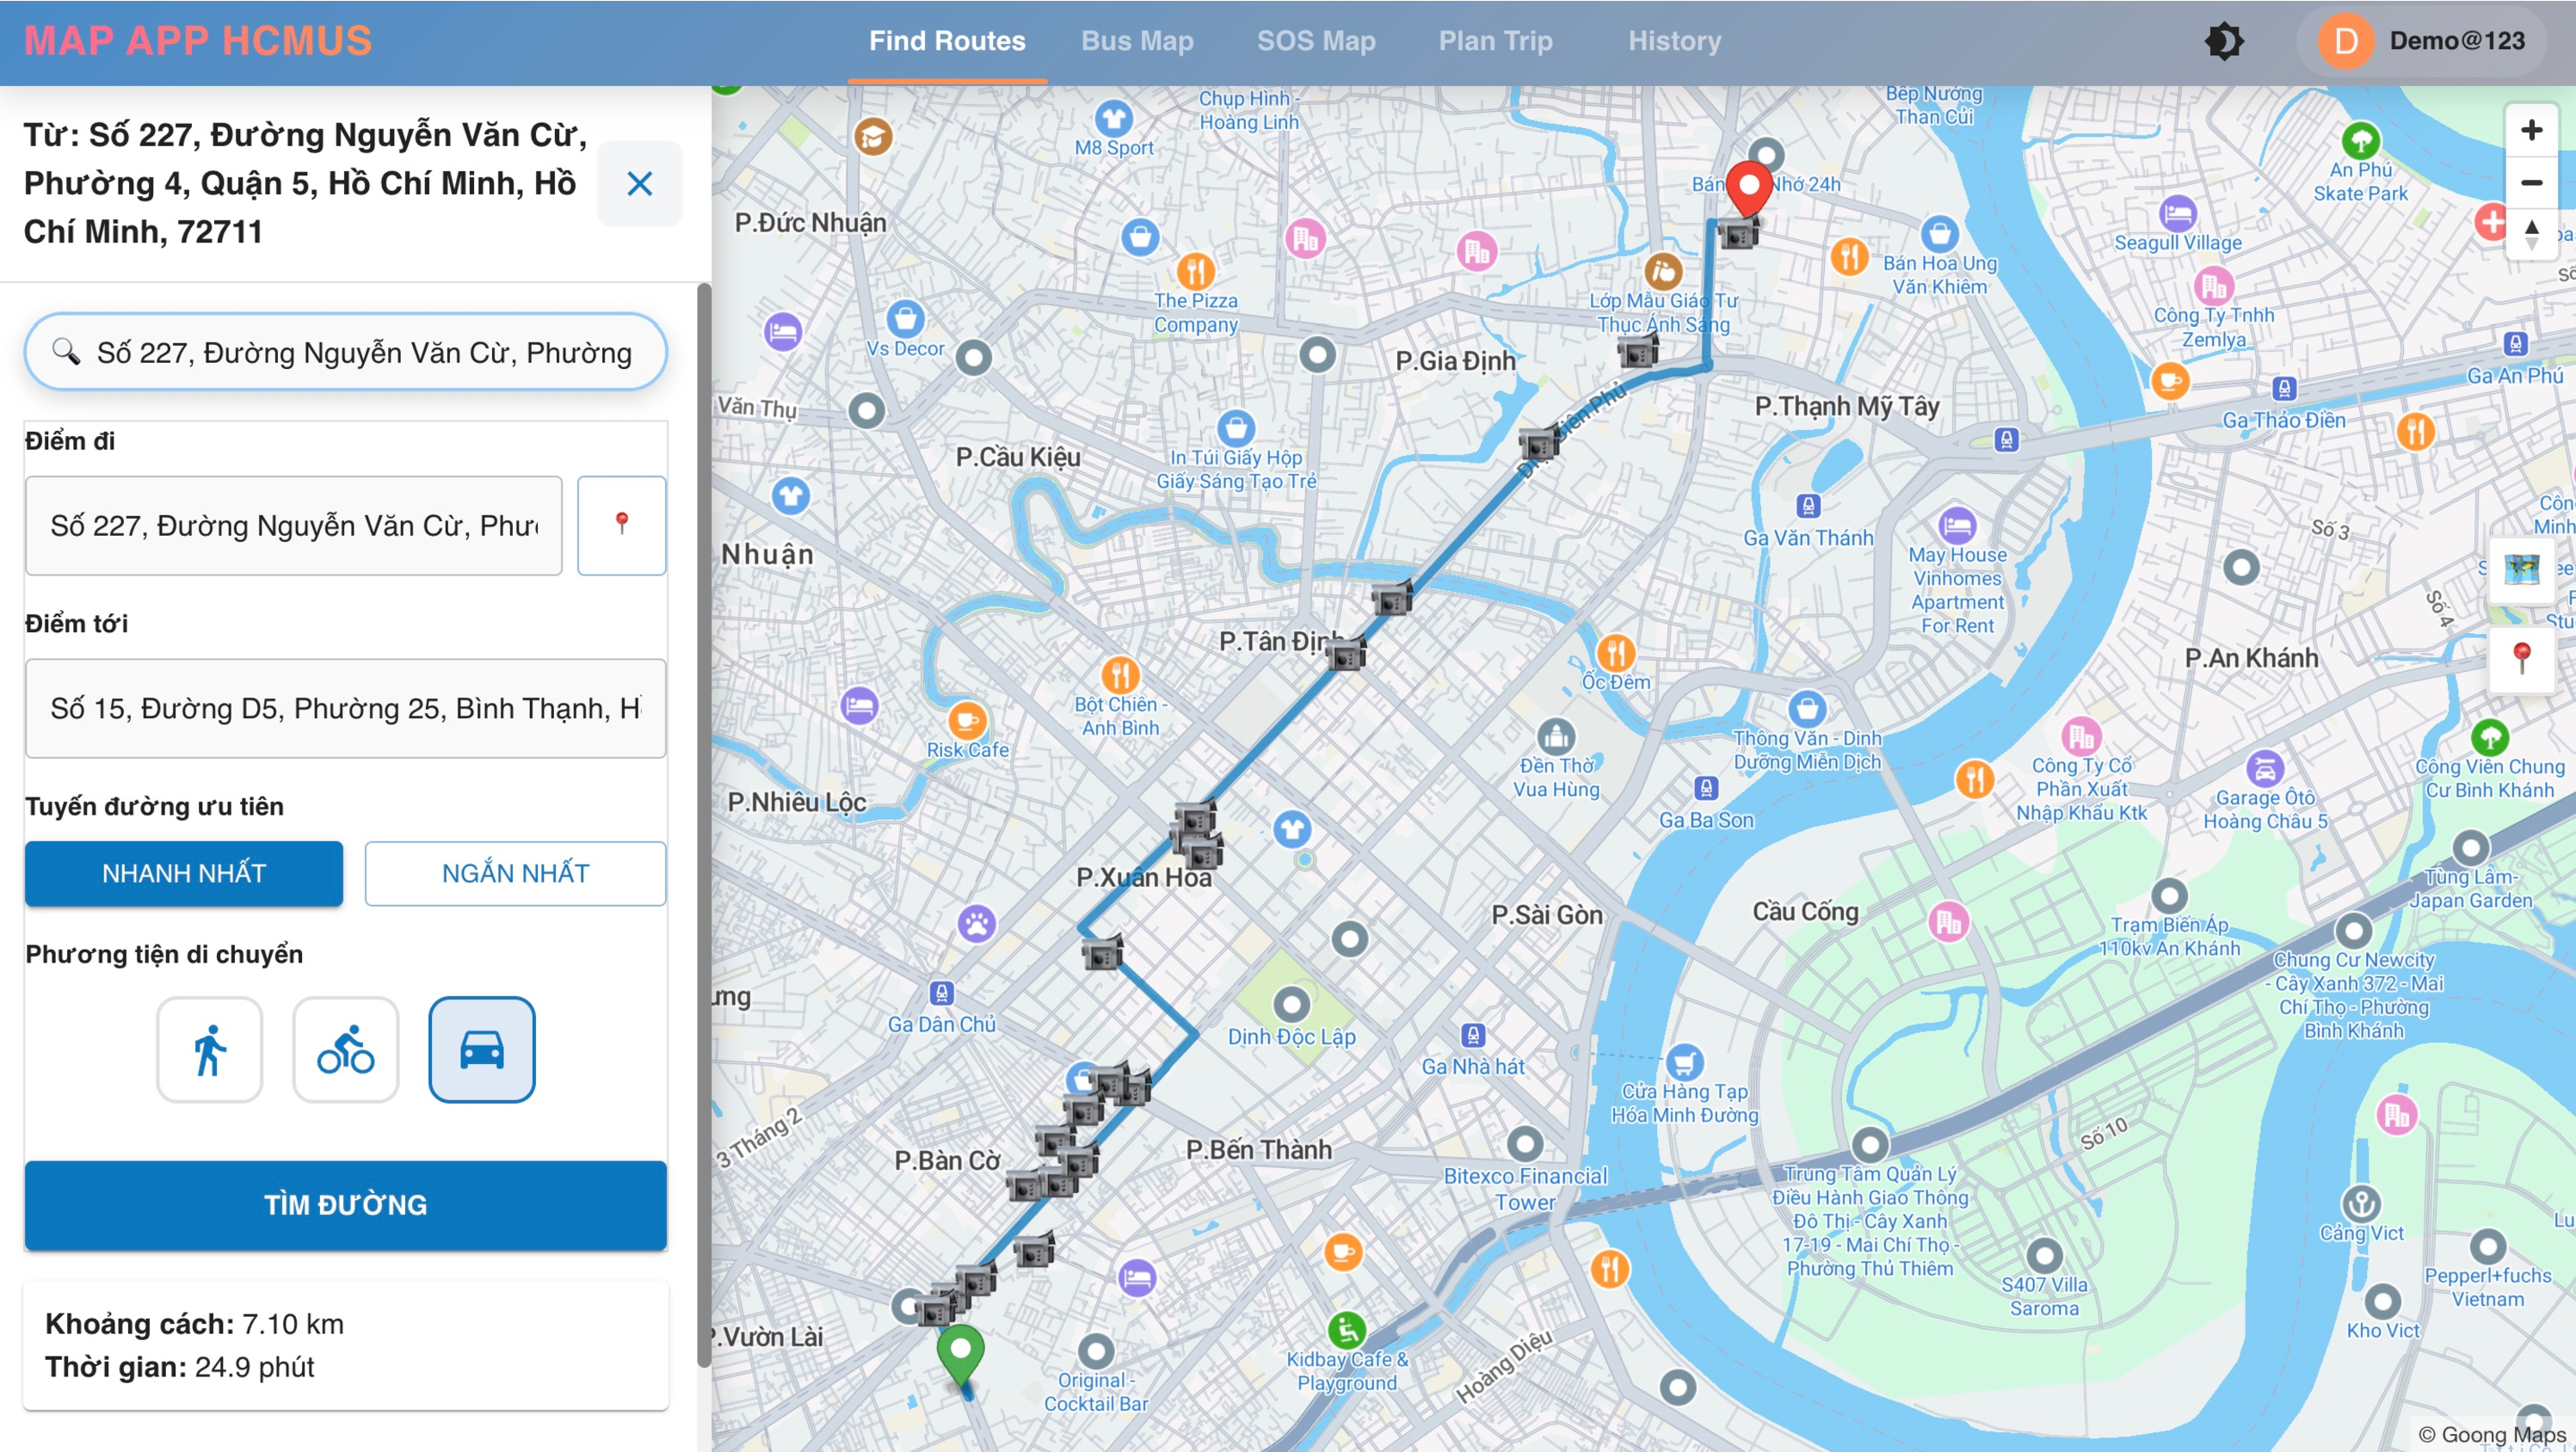
\includegraphics[width=1\textwidth]{figures/Route_Planning_Page.pdf}
    \caption{Route Planning Interface}
    \label{fig:screenshot-routes}
\end{figure}
Users can search for locations, select transport mode, and view routes with color-coded congestion (blue/yellow/red)

\begin{figure}[H]
    \centering
    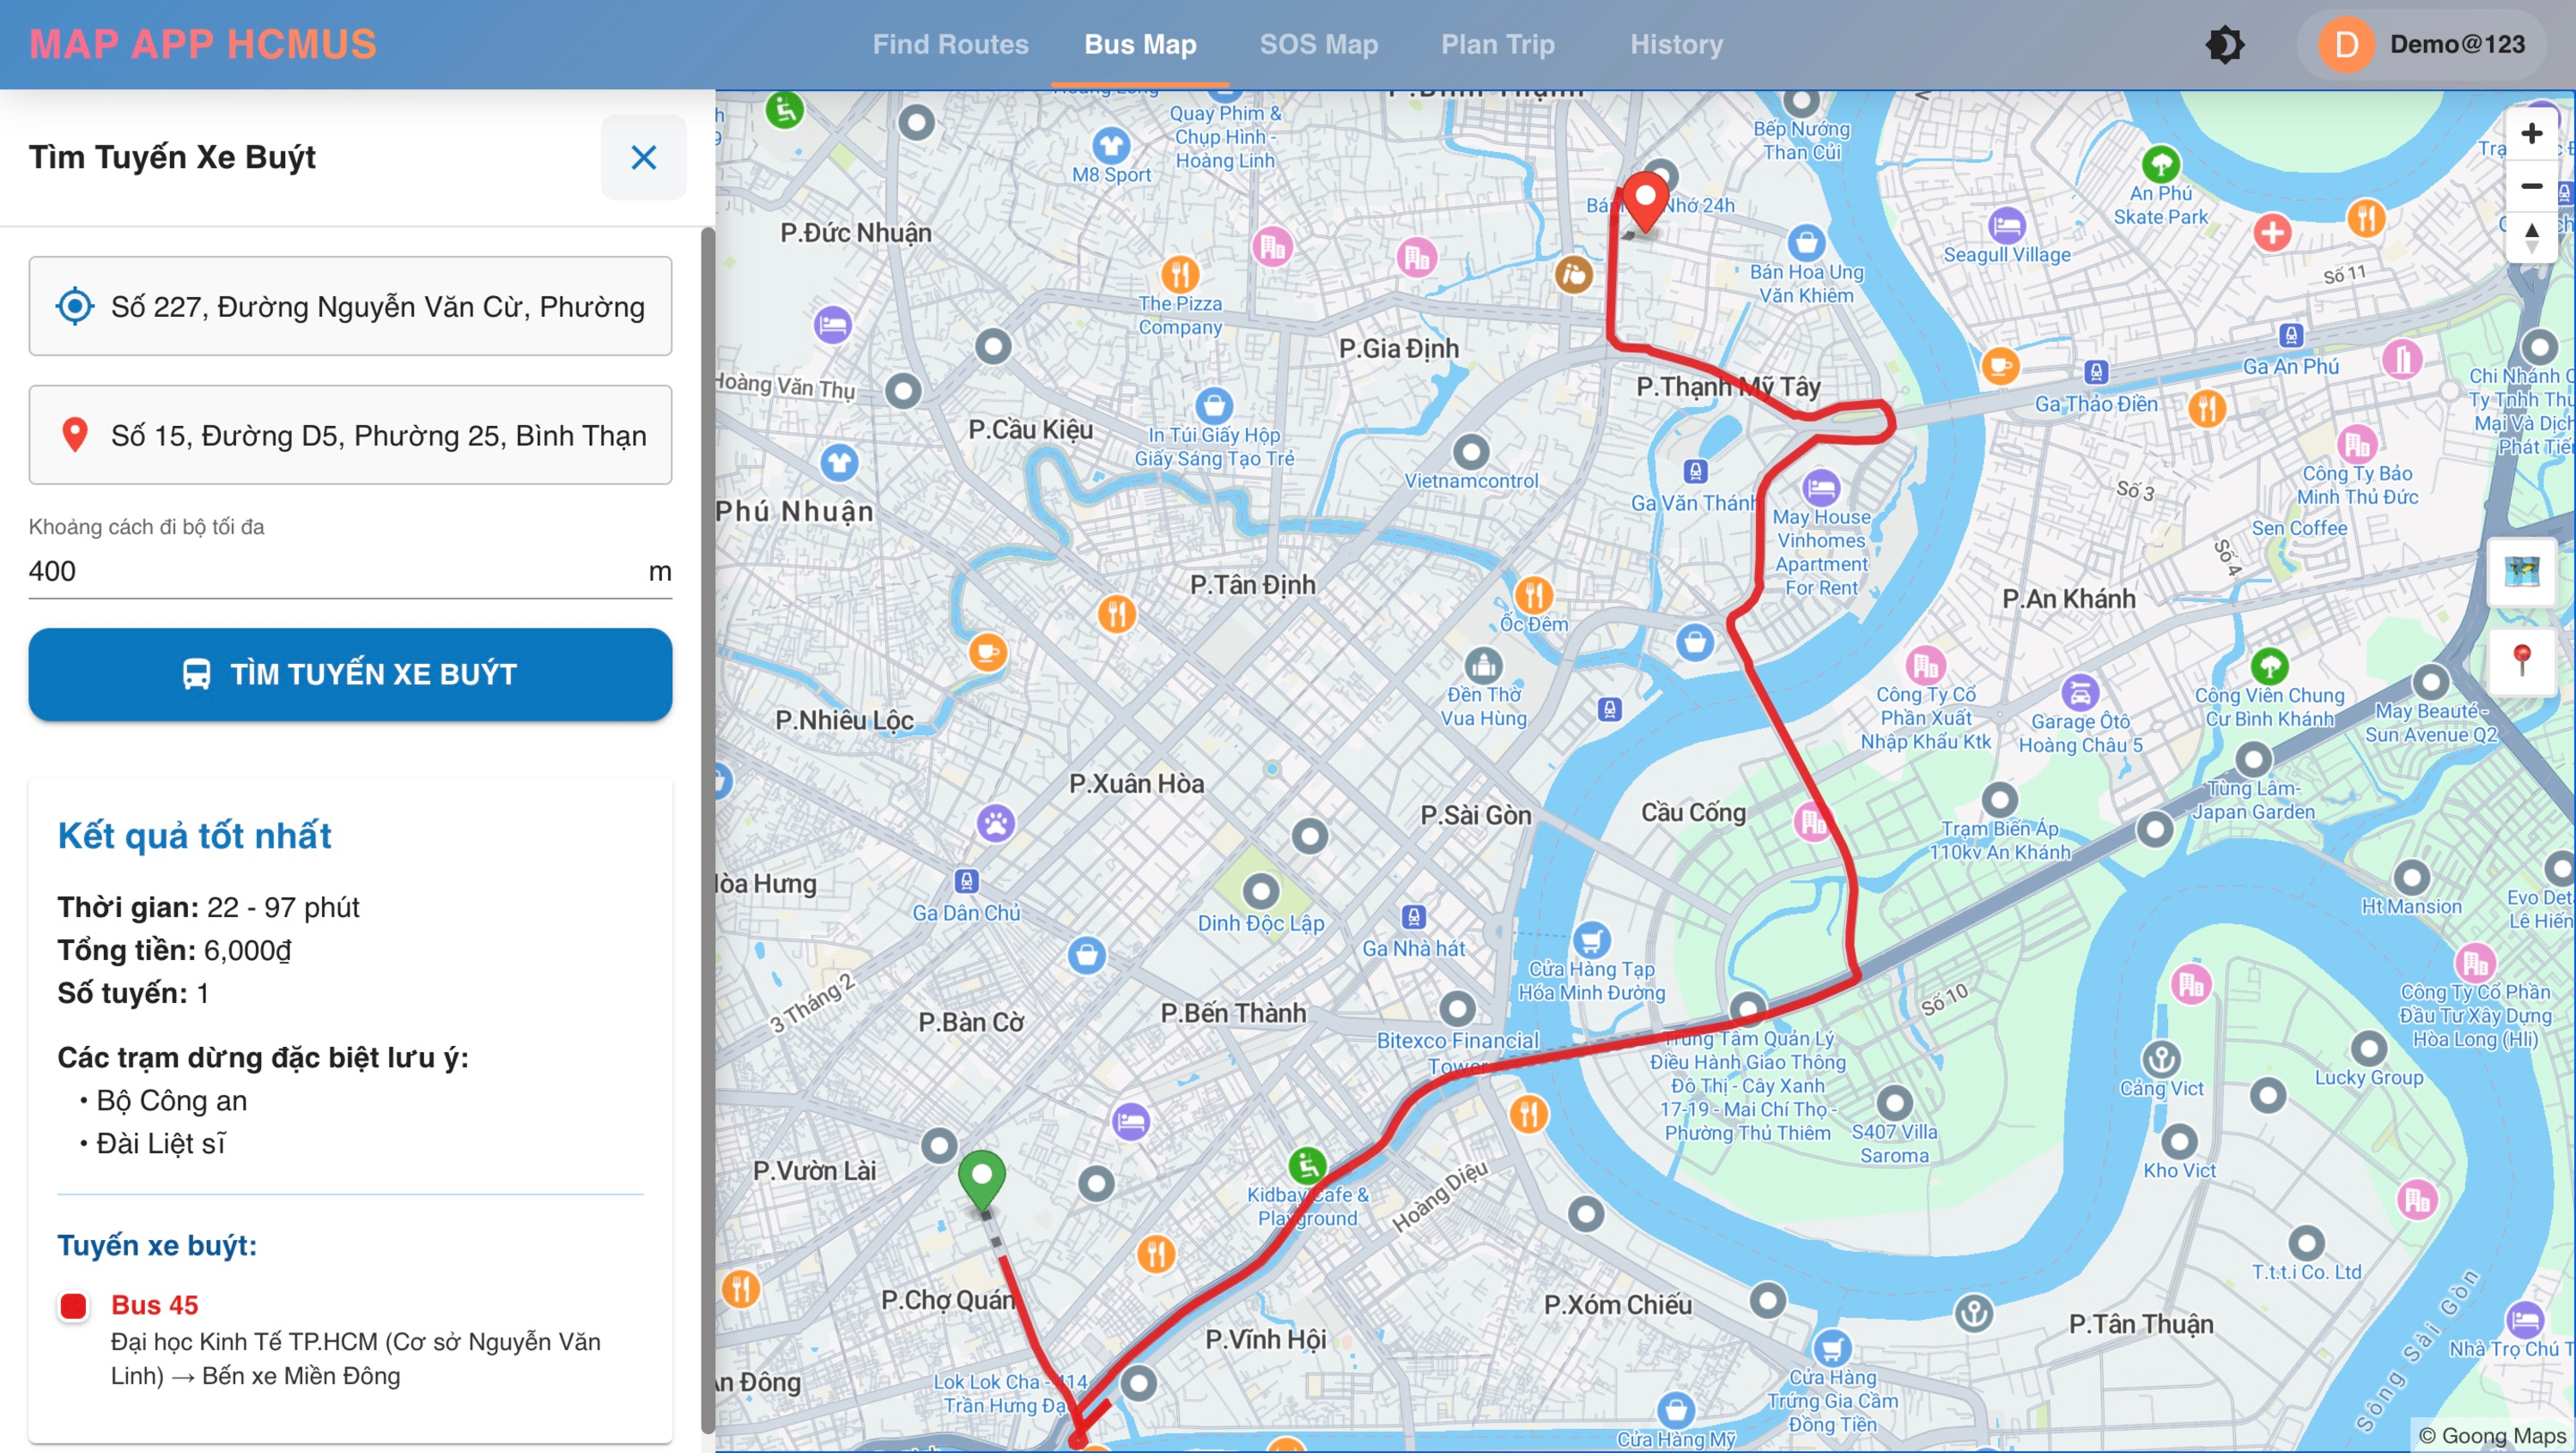
\includegraphics[width=1\textwidth]{figures/Bus_Routing_Page.pdf}
    \caption{Bus Routing Interface}
    \label{fig:screenshot-bus}
\end{figure}
Displays optimal bus routes with transfer points, walking segments, and estimated travel times

\begin{figure}[H]
    \centering
    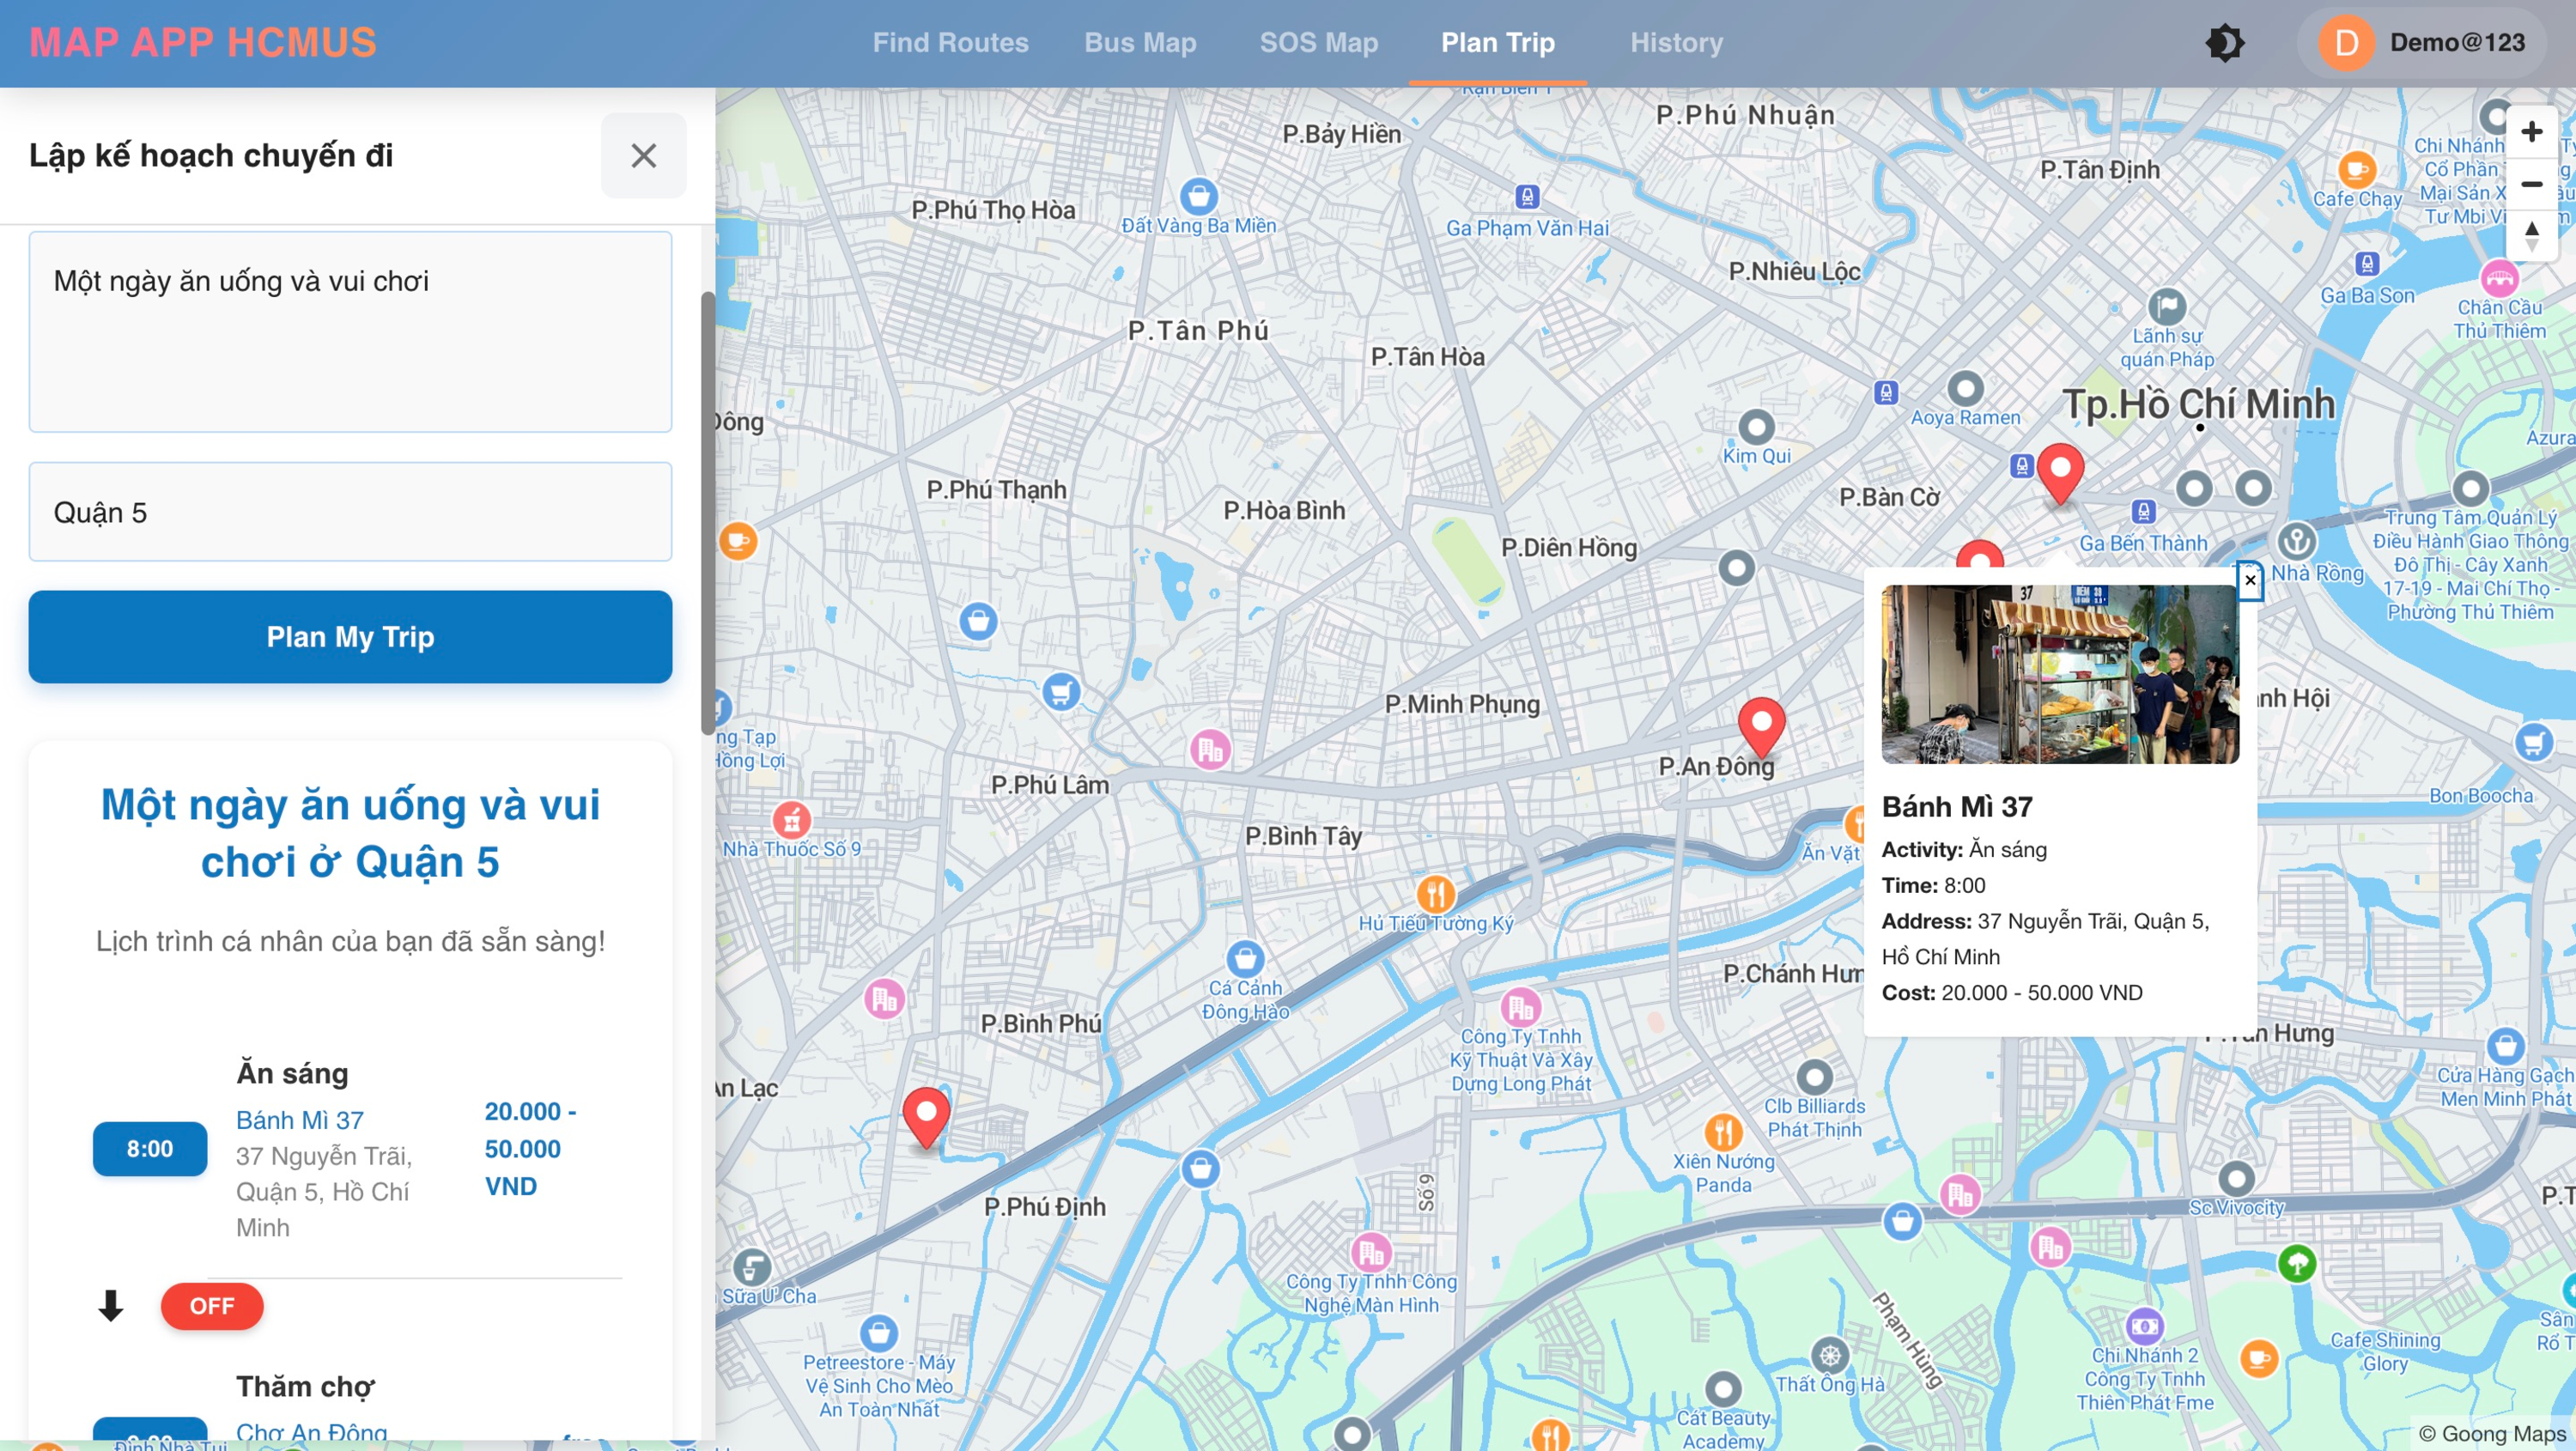
\includegraphics[width=1\textwidth]{figures/AI_Trip_Planner_Page.pdf}
    \caption{AI Trip Planner}
    \label{fig:screenshot-trip}
\end{figure}
Users enter queries like ``\VN{Một ngày ăn uống và vui chơi}'' and receive complete itineraries with numbered markers

\begin{figure}[H]
    \centering
    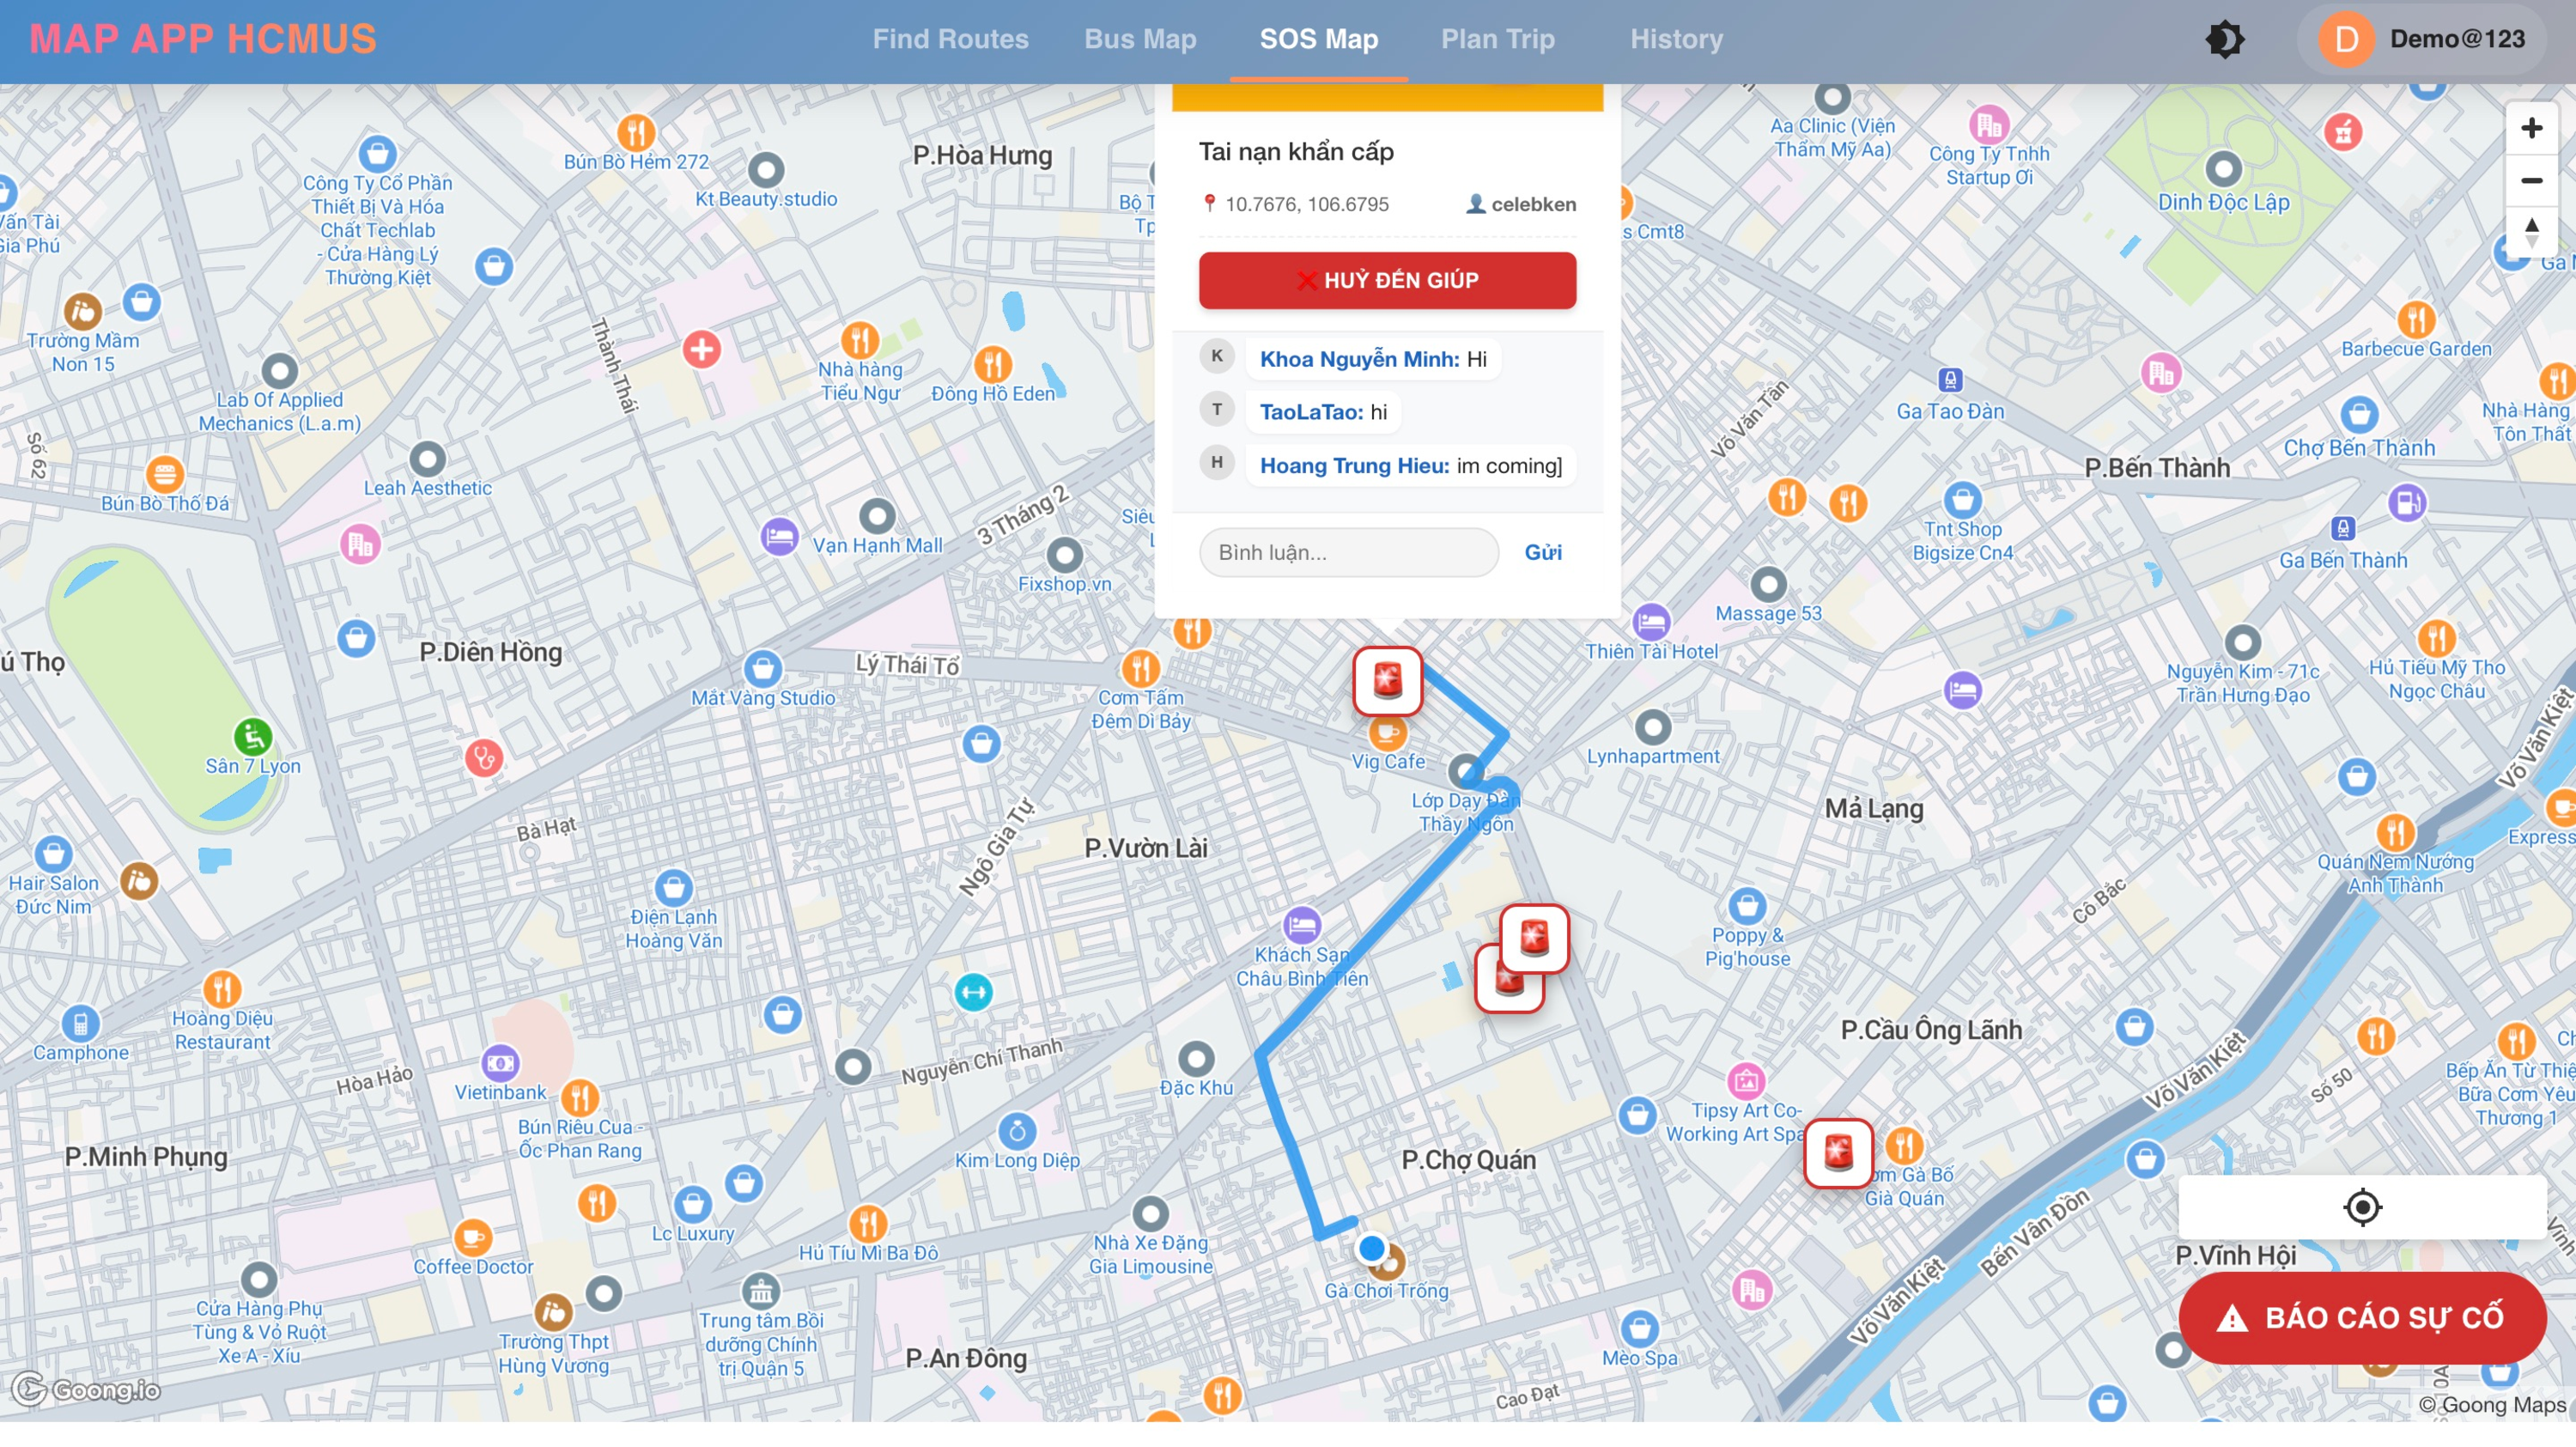
\includegraphics[width=1\textwidth]{figures/SOS_Emergency_Map.pdf}
    \caption{SOS Emergency System}
\end{figure}
Community-driven incident reporting with image upload, comments, and spam prevention

\begin{figure}[H]
    \centering
    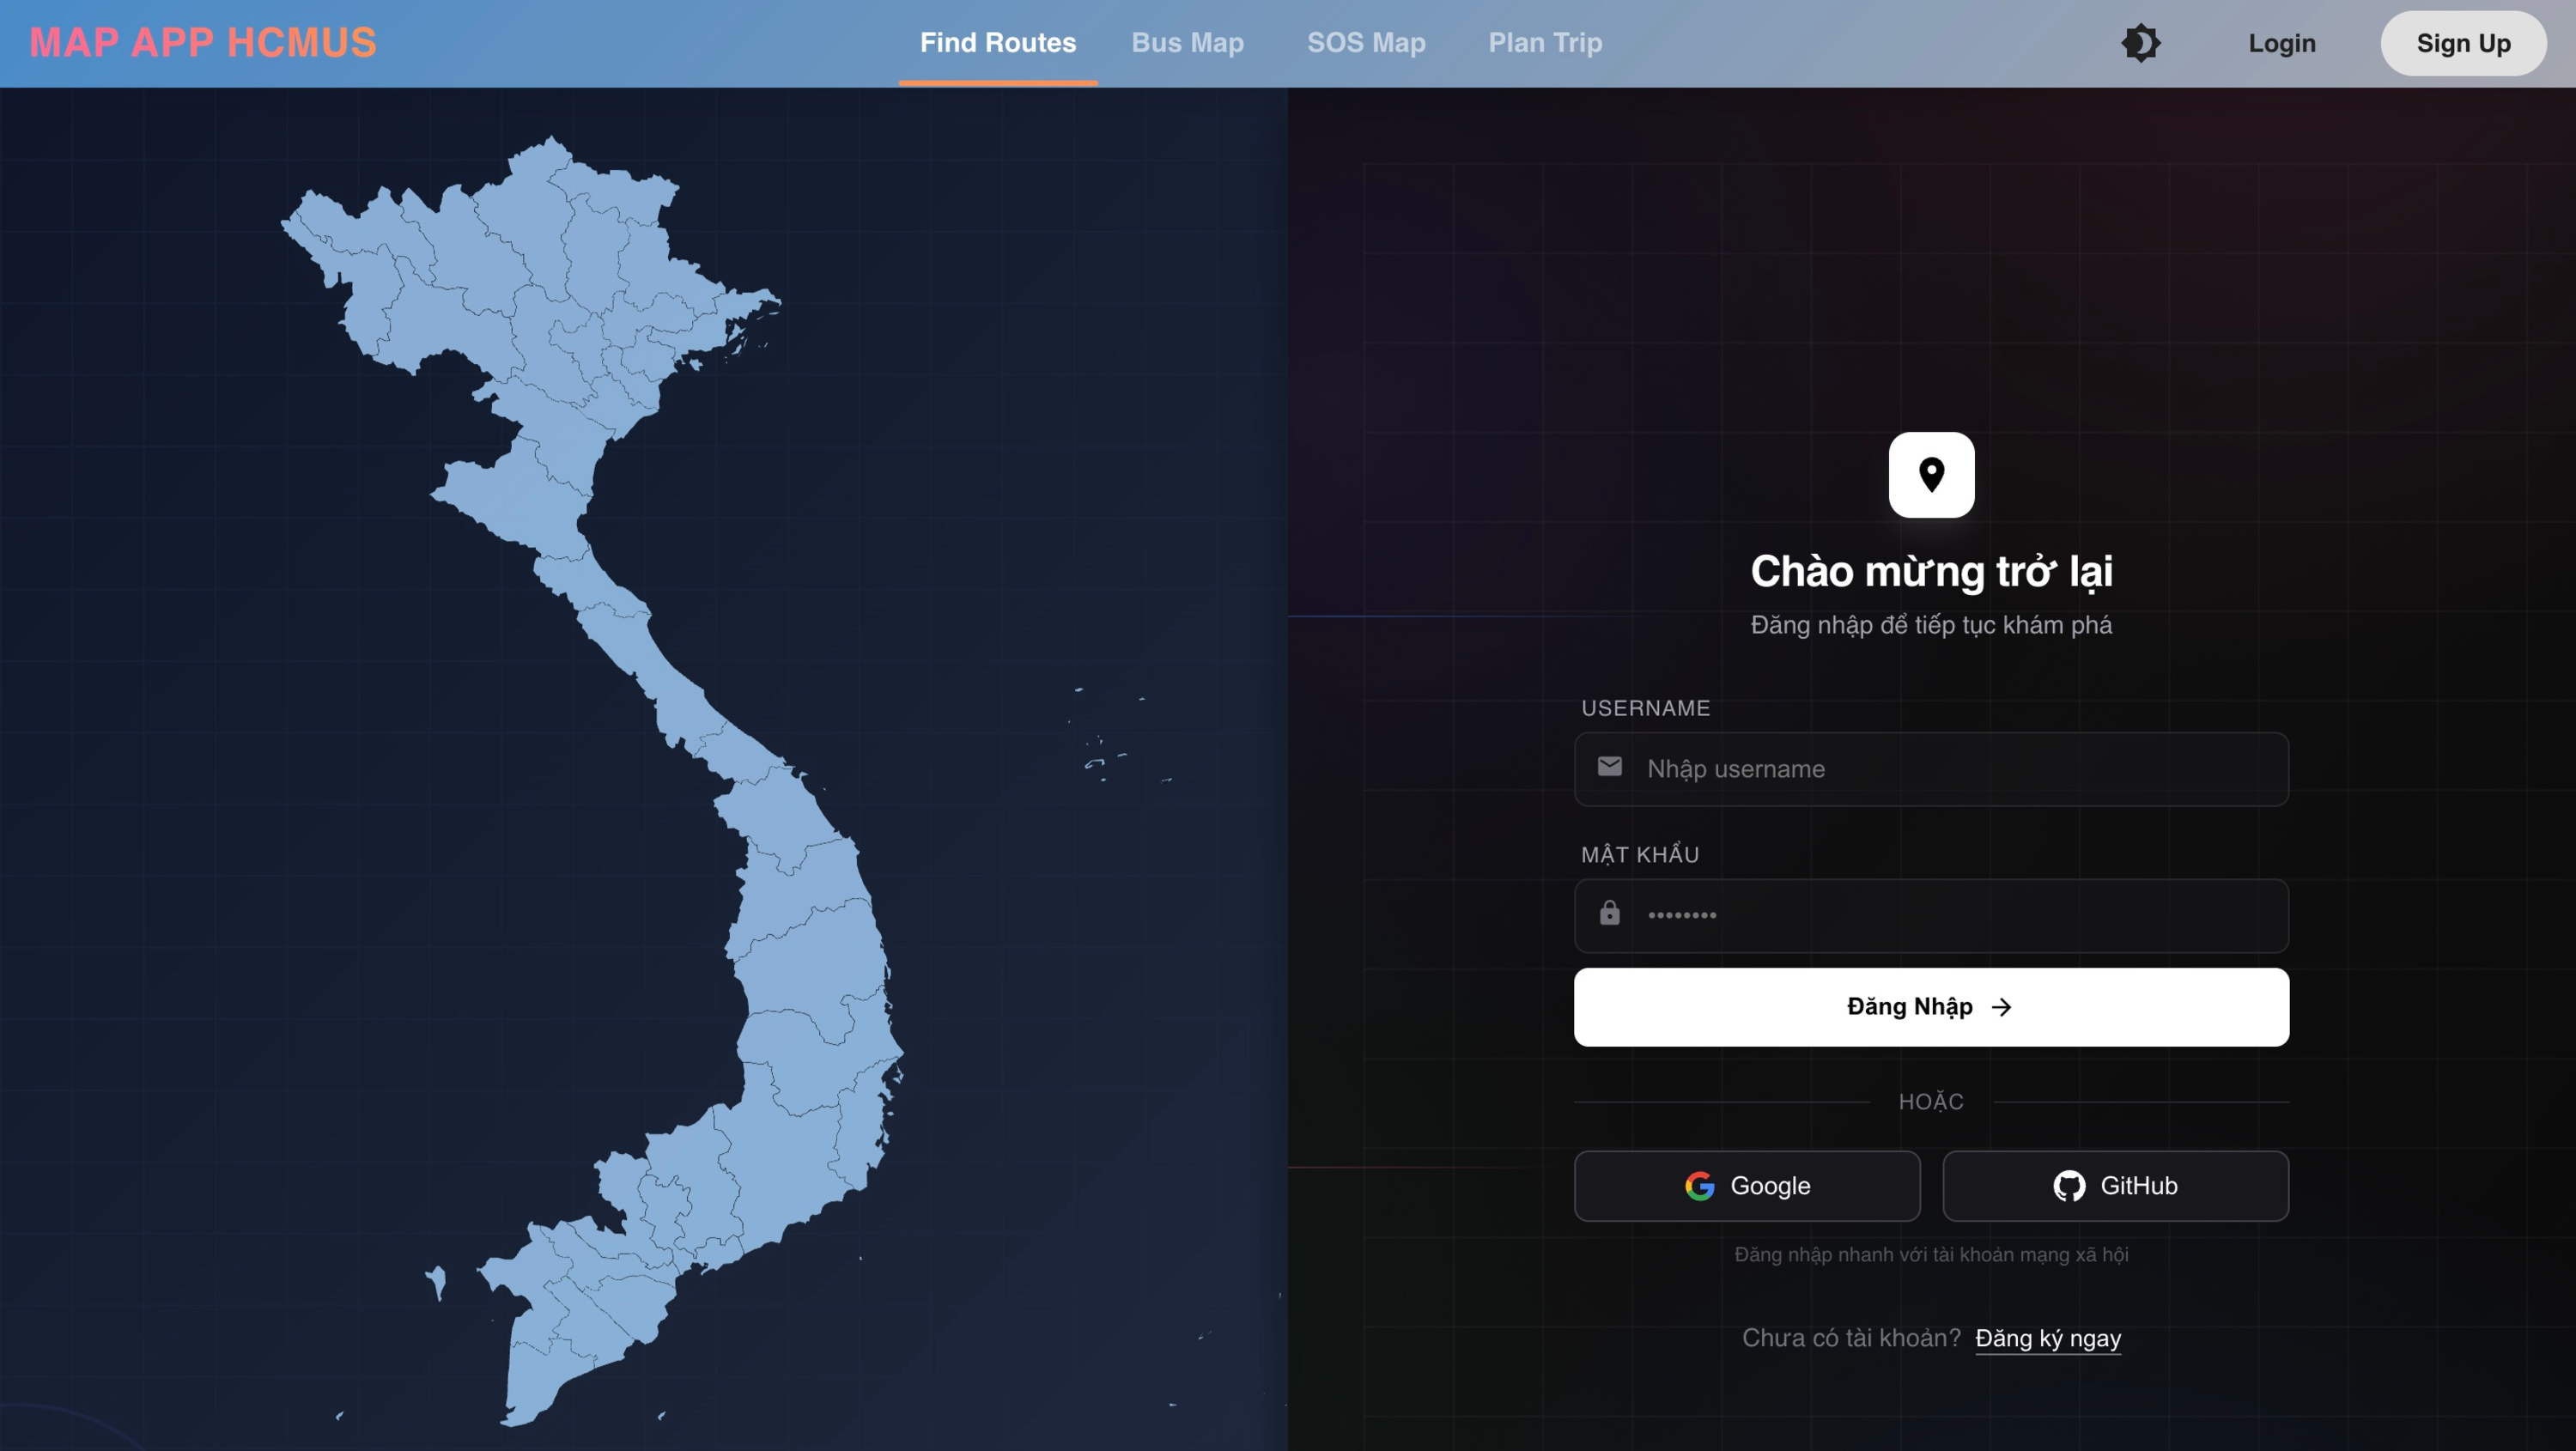
\includegraphics[width=1\textwidth]{figures/Login:Authentication_Page.pdf}
    \caption{Authentication Interface}
    \label{fig:screenshot-login}
\end{figure}
Secure login with traditional credentials or OAuth providers (Google, GitHub)